\documentclass[11pt]{article}
\usepackage[margin=0.5in]{geometry}
\usepackage{tikz}
\usetikzlibrary{calc, decorations.markings, arrows.meta}

\begin{document}

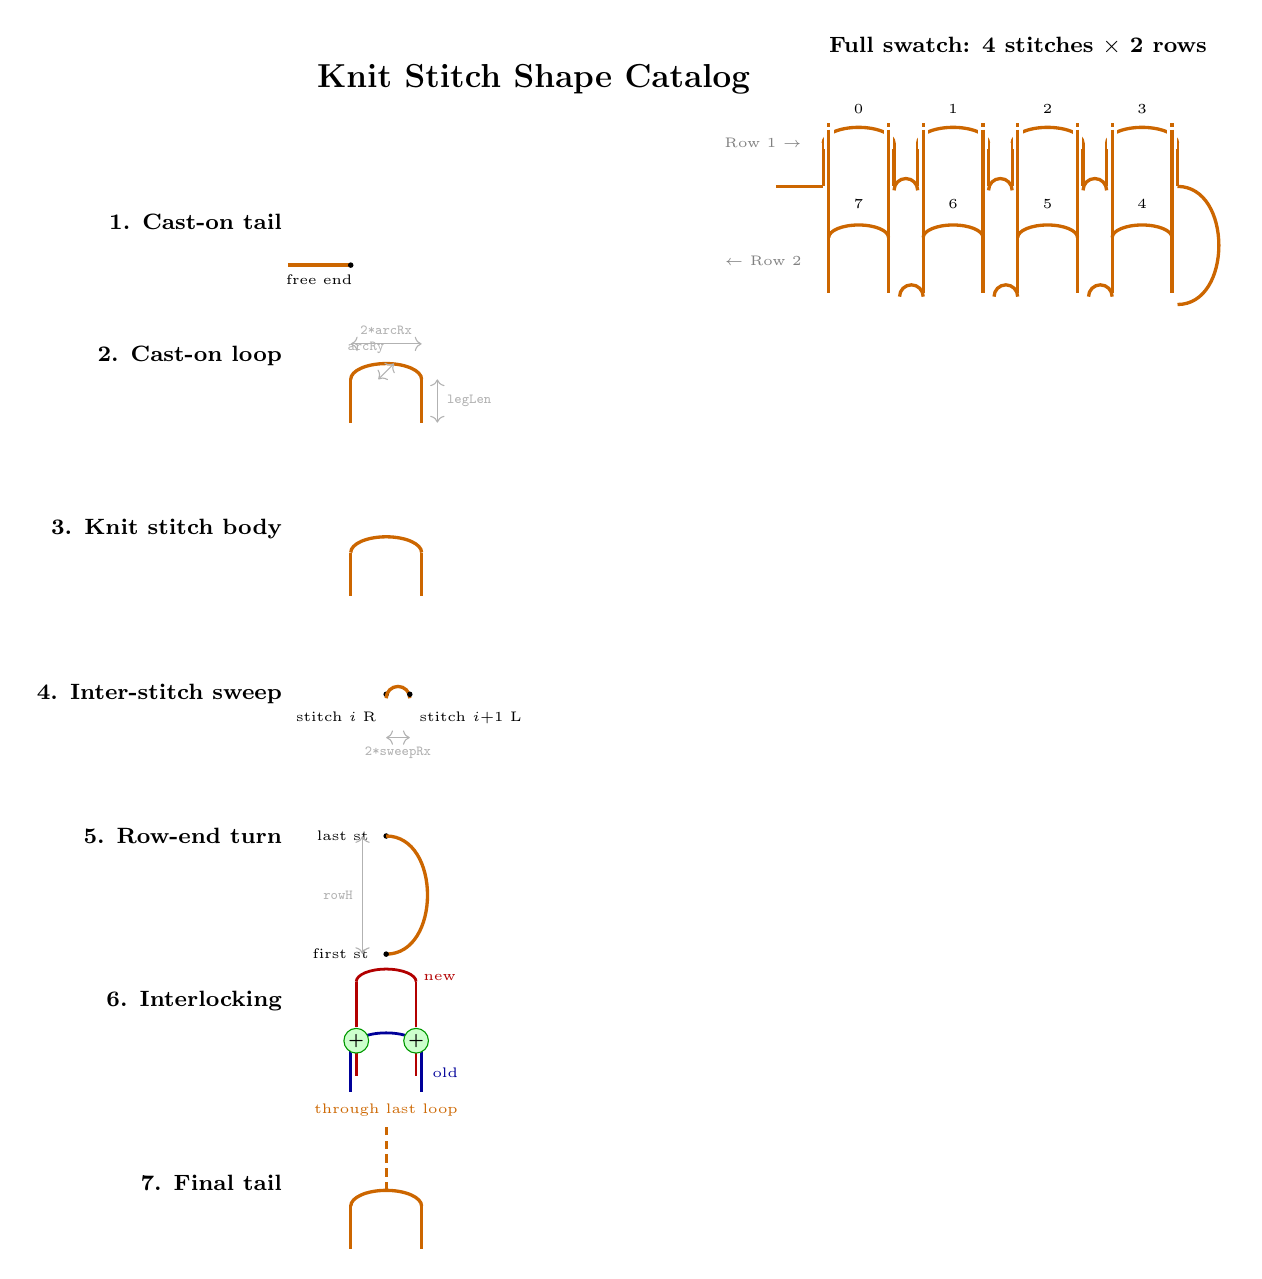
\begin{tikzpicture}[
  % ================================================================
  % TUNABLE PARAMETERS — adjust these to control the stitch geometry
  % ================================================================
]

% --- Stitch shape parameters ---
\pgfmathsetmacro{\arcRx}{0.45}      % half-width of upper ellipse
\pgfmathsetmacro{\arcRy}{0.20}      % half-height of upper ellipse
\pgfmathsetmacro{\legLen}{0.55}     % length of straight legs below tangent
\pgfmathsetmacro{\legGap}{0.05}     % gap between leg bottom and sweep arc
\pgfmathsetmacro{\sweepRx}{0.15}    % half-width of inter-stitch sweep arc
\pgfmathsetmacro{\sweepRy}{0.15}    % half-height of inter-stitch sweep arc

% --- Layout parameters ---
\pgfmathsetmacro{\stitchW}{1.2}     % horizontal center-to-center spacing
\pgfmathsetmacro{\rowH}{1.5}        % vertical center-to-center row spacing
\pgfmathsetmacro{\turnBulge}{0.7}   % how far the row-end turn sticks out

% --- Derived values ---
\pgfmathsetmacro{\legBot}{-\legLen}          % y of leg bottom relative to arc center
\pgfmathsetmacro{\sweepBot}{\legBot-\legGap} % y of sweep arc center

% --- Style ---
\tikzset{
  yarn/.style={line width=1.2pt, orange!80!black},
  yarn thin/.style={line width=0.8pt, orange!80!black},
  gap/.style={line width=3.5pt, white},  % white overprint for crossings
  crossing mark/.style={fill=green!20, draw=green!60!black,
    circle, inner sep=0.5pt, font=\tiny, minimum size=6pt},
}

% ================================================================
% SHAPE CATALOG
% ================================================================

\node[anchor=south west, font=\large\bfseries] at (-1, 1.5) {Knit Stitch Shape Catalog};

% --- 1. Cast-on tail ---
\node[anchor=east, font=\footnotesize\bfseries] at (-1.2, 0) {1. Cast-on tail};
\draw[yarn] ({-\arcRx - 0.8}, \legBot) -- ({-\arcRx}, \legBot);
\fill[black] ({-\arcRx}, \legBot) circle(1pt);
\node[font=\tiny, below] at ({-\arcRx - 0.4}, \legBot) {free end};

% --- 2. Cast-on loop ---
\begin{scope}[shift={(0, -2)}]
\node[anchor=east, font=\footnotesize\bfseries] at (-1.2, 0.3) {2. Cast-on loop};
% Upper arc
\draw[yarn] ({-\arcRx}, 0)
  arc[start angle=180, end angle=0, x radius=\arcRx, y radius=\arcRy];
% Left leg
\draw[yarn] ({-\arcRx}, 0) -- ({-\arcRx}, \legBot);
% Right leg
\draw[yarn] ({\arcRx}, 0) -- ({\arcRx}, \legBot);
% Dimension annotations
\draw[<->, thin, gray!60] ({-\arcRx}, 0.45) -- ({\arcRx}, 0.45)
  node[midway, above, font=\tiny\ttfamily] {2*arcRx};
\draw[<->, thin, gray!60] ({\arcRx+0.2}, 0) -- ({\arcRx+0.2}, \legBot)
  node[midway, right, font=\tiny\ttfamily] {legLen};
\draw[<->, thin, gray!60] ({-0.1}, 0) -- ({0.1}, \arcRy)
  node[above left, font=\tiny\ttfamily] {arcRy};
\end{scope}

% --- 3. Knit stitch body ---
\begin{scope}[shift={(0, -4.2)}]
\node[anchor=east, font=\footnotesize\bfseries] at (-1.2, 0.3) {3. Knit stitch body};
% Upper arc
\draw[yarn] ({-\arcRx}, 0)
  arc[start angle=180, end angle=0, x radius=\arcRx, y radius=\arcRy];
% Left leg
\draw[yarn] ({-\arcRx}, 0) -- ({-\arcRx}, \legBot);
% Right leg
\draw[yarn] ({\arcRx}, 0) -- ({\arcRx}, \legBot);
\end{scope}

% --- 4. Inter-stitch sweep ---
\begin{scope}[shift={(0, -6.0)}]
\node[anchor=east, font=\footnotesize\bfseries] at (-1.2, 0) {4. Inter-stitch sweep};
% Right leg bottom of stitch N
\fill[black] (0, 0) circle(1pt);
\node[font=\tiny, below left] at (0, -0.1) {stitch $i$ R};
% Sweep arc to next stitch
\draw[yarn] (0, {-\legGap})
  arc[start angle=180, end angle=0, x radius=\sweepRx, y radius=\sweepRy];
% Left leg bottom of stitch N+1
\fill[black] ({2*\sweepRx}, 0) circle(1pt);
\node[font=\tiny, below right] at ({2*\sweepRx}, -0.1) {stitch $i{+}1$ L};
% Dimension
\draw[<->, thin, gray!60] (0, -0.55) -- ({2*\sweepRx}, -0.55)
  node[midway, below, font=\tiny\ttfamily] {2*sweepRx};
\end{scope}

% --- 5. Row-end turn ---
\begin{scope}[shift={(0, -7.8)}]
\node[anchor=east, font=\footnotesize\bfseries] at (-1.2, 0) {5. Row-end turn};
\fill[black] (0, 0) circle(1pt);
\node[font=\tiny, left] at (-0.1, 0) {last st};
% Bezier U-turn
\draw[yarn] (0, 0)
  .. controls ({\turnBulge}, 0) and ({\turnBulge}, {-\rowH}) ..
  (0, {-\rowH});
\fill[black] (0, {-\rowH}) circle(1pt);
\node[font=\tiny, left] at (-0.1, {-\rowH}) {first st};
\draw[<->, thin, gray!60] ({-0.3}, 0) -- ({-0.3}, {-\rowH})
  node[midway, left, font=\tiny\ttfamily] {rowH};
\end{scope}

% --- 6. Interlocking crossing ---
\begin{scope}[shift={(0, -10.5)}]
\node[anchor=east, font=\footnotesize\bfseries] at (-1.2, 0.6) {6. Interlocking};

% OLD stitch (row below) — blue
\draw[yarn, blue!60!black, line width=1pt] ({-\arcRx}, 0)
  arc[start angle=180, end angle=0, x radius=\arcRx, y radius=\arcRy];
\draw[yarn, blue!60!black, line width=1pt] ({-\arcRx}, 0)
  -- ({-\arcRx}, \legBot);
\draw[yarn, blue!60!black, line width=1pt] ({\arcRx}, 0)
  -- ({\arcRx}, \legBot);

% NEW stitch (row above) — red, its legs pass through old loop
% New stitch arc sits above old stitch
\pgfmathsetmacro{\newY}{0.85}
\pgfmathsetmacro{\newRx}{0.38}
\pgfmathsetmacro{\newRy}{0.16}

\draw[yarn, red!70!black, line width=1pt] ({-\newRx}, \newY)
  arc[start angle=180, end angle=0, x radius=\newRx, y radius=\newRy];

% New left leg: comes down, crosses old arc
% Above crossing
\draw[yarn, red!70!black, line width=1pt] ({-\newRx}, \newY)
  -- ({-\newRx}, {\arcRy + 0.08});
% White gap over old arc
\draw[gap] ({-\newRx}, \arcRy) -- ({-\newRx}, {-0.05});
% Below crossing (continues down)
\draw[yarn, red!70!black, line width=1pt] ({-\newRx}, {\arcRy - 0.02})
  -- ({-\newRx}, {-0.35});

% New right leg
\draw[yarn, red!70!black, line width=1pt] ({\newRx}, \newY)
  -- ({\newRx}, {\arcRy + 0.08});
\draw[gap] ({\newRx}, \arcRy) -- ({\newRx}, {-0.05});
\draw[yarn, red!70!black, line width=1pt] ({\newRx}, {\arcRy - 0.02})
  -- ({\newRx}, {-0.35});

% Crossing markers
\node[crossing mark] at ({-\newRx}, {\arcRy*0.5}) {\textbf{+}};
\node[crossing mark] at ({\newRx}, {\arcRy*0.5}) {\textbf{+}};

\node[font=\tiny, blue!60!black] at ({\arcRx+0.3}, -0.3) {old};
\node[font=\tiny, red!70!black] at ({\newRx+0.3}, 0.9) {new};
\end{scope}

% --- 7. Final tail ---
\begin{scope}[shift={(0, -12.5)}]
\node[anchor=east, font=\footnotesize\bfseries] at (-1.2, 0.3) {7. Final tail};
\draw[yarn] ({-\arcRx}, 0)
  arc[start angle=180, end angle=0, x radius=\arcRx, y radius=\arcRy];
\draw[yarn] ({-\arcRx}, 0) -- ({-\arcRx}, \legBot);
\draw[yarn] ({\arcRx}, 0) -- ({\arcRx}, \legBot);
% Tail going through and out
\draw[yarn, densely dashed] (0, \arcRy) -- (0, {1.0})
  node[above, font=\tiny] {through last loop};
\end{scope}

% ================================================================
% COMBINED: Full 4-stitch x 2-row stockinette swatch
% ================================================================
\begin{scope}[shift={(6, 1)}]
\node[anchor=south west, font=\footnotesize\bfseries]
  at (-0.5, 1) {Full swatch: 4 stitches $\times$ 2 rows};

% --- Cast-on tail ---
\draw[yarn] ({-\arcRx - 0.6}, \legBot) -- ({-\arcRx}, \legBot);

% --- ROW 1: Cast-on, 4 stitches left to right ---
\foreach \i in {0,1,2,3} {
  \pgfmathsetmacro{\cx}{\i * \stitchW}
  % Upper arc
  \draw[yarn] ({\cx - \arcRx}, 0)
    arc[start angle=180, end angle=0, x radius=\arcRx, y radius=\arcRy];
  % Left leg
  \draw[yarn] ({\cx - \arcRx}, 0) -- ({\cx - \arcRx}, \legBot);
  % Right leg
  \draw[yarn] ({\cx + \arcRx}, 0) -- ({\cx + \arcRx}, \legBot);
}

% Inter-stitch sweeps for row 1
\foreach \i in {0,1,2} {
  \pgfmathsetmacro{\sx}{\i * \stitchW + \arcRx}
  \draw[yarn] ({\sx}, {\legBot - \legGap})
    arc[start angle=180, end angle=0, x radius=\sweepRx, y radius=\sweepRy];
}

% --- Row-end turn (right side) ---
\pgfmathsetmacro{\lastX}{3 * \stitchW + \arcRx}
\draw[yarn] ({\lastX}, \legBot)
  .. controls ({\lastX + \turnBulge}, \legBot)
  and ({\lastX + \turnBulge}, {\legBot - \rowH}) ..
  ({\lastX}, {\legBot - \rowH});

% --- ROW 2: 4 stitches right to left, interlocking with row 1 ---
\pgfmathsetmacro{\ryTwo}{-\rowH}  % y-offset for row 2 arc centers

\foreach \i in {0,1,2,3} {
  \pgfmathsetmacro{\cx}{\i * \stitchW}
  \pgfmathsetmacro{\newArcY}{\ryTwo + \arcRy + 0.1}

  % New stitch upper arc (within row 1's stitch legs)
  \pgfmathsetmacro{\nRx}{0.38}
  \pgfmathsetmacro{\nRy}{0.16}
  \draw[yarn] ({\cx + \nRx}, \newArcY)
    arc[start angle=0, end angle=180, x radius=\nRx, y radius=\nRy];

  % Left leg of new stitch — passes through old loop
  % Above the crossing
  \draw[yarn] ({\cx - \nRx}, \newArcY) -- ({\cx - \nRx}, {\arcRy + 0.05});
  % Gap in old stitch's arc
  \draw[gap] ({\cx - \nRx}, {\arcRy}) -- ({\cx - \nRx}, {-0.07});
  % Below crossing
  \draw[yarn] ({\cx - \nRx}, {\arcRy - 0.03})
    -- ({\cx - \nRx}, {\ryTwo - \legLen + 0.15});

  % Right leg of new stitch
  \draw[yarn] ({\cx + \nRx}, \newArcY) -- ({\cx + \nRx}, {\arcRy + 0.05});
  \draw[gap] ({\cx + \nRx}, {\arcRy}) -- ({\cx + \nRx}, {-0.07});
  \draw[yarn] ({\cx + \nRx}, {\arcRy - 0.03})
    -- ({\cx + \nRx}, {\ryTwo - \legLen + 0.15});
}

% Inter-stitch sweeps for row 2 (going right to left)
\foreach \i in {0,1,2} {
  \pgfmathsetmacro{\sx}{(\i + 1) * \stitchW - 0.38}
  \draw[yarn] ({\sx}, {\ryTwo - \legLen + 0.15 - \legGap})
    arc[start angle=0, end angle=180, x radius=\sweepRx, y radius=\sweepRy];
}

% Row labels
\node[font=\tiny, gray, anchor=east] at (-0.6, 0) {Row 1 $\to$};
\node[font=\tiny, gray, anchor=east] at (-0.6, \ryTwo) {$\leftarrow$ Row 2};

% Stitch index labels
\foreach \i in {0,1,2,3} {
  \pgfmathsetmacro{\cx}{\i * \stitchW}
  \node[font=\tiny, above] at (\cx, \arcRy + 0.05) {\i};
}
\foreach \i [count=\j from 0] in {7,6,5,4} {
  \pgfmathsetmacro{\cx}{\j * \stitchW}
  \pgfmathsetmacro{\ly}{\ryTwo + \arcRy + 0.35}
  \node[font=\tiny, above] at (\cx, \ly) {\i};
}

\end{scope}

\end{tikzpicture}

\end{document}
